\documentclass[tikz]{standalone}
\usepackage{lmodern}
\usepackage[algoruled,vlined,linesnumbered,titlenotnumbered,noend]{algorithm2e}
\usepackage{color,amsmath,bm,bbm,stmaryrd,amssymb,pifont,bbding}
\usetikzlibrary{backgrounds}
\usetikzlibrary{calc} 

\usetikzlibrary{shapes}
\usetikzlibrary{shadows}
\usetikzlibrary{decorations.pathmorphing}
\usetikzlibrary{decorations.text}
\usetikzlibrary{decorations}
\usetikzlibrary{arrows,bending}
\usetikzlibrary{shapes.arrows}
\tikzset{nobg/.style={show background rectangle,background rectangle/.style={opacity=0}}}


%\input ../../styles
%\input ../../globalcomm
\usetikzlibrary{arrows, shapes.gates.logic.US, calc}

\begin{document}
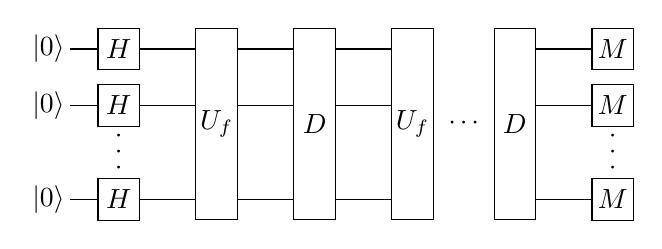
\begin{tikzpicture}
\node[draw,name=h0,inner sep=0pt,minimum size=15pt] 
at (0,0){$H$};
\node[draw,name=h1,inner sep=0pt,minimum size=15pt,anchor=north] 
at($(h0.south)+(0pt,-5pt)$){$H$};
\node[name=cdot1,inner sep=0pt,anchor=north] 
at($(h1.south)+(0pt,-1pt)$){$\cdot$};
\node[name=cdot2,inner sep=0pt,anchor=north] 
at($(cdot1.south)+(0pt,-1pt)$){$\cdot$};
\node[name=cdot3,inner sep=0pt,anchor=north] 
at($(cdot2.south)+(0pt,-1pt)$){$\cdot$};
\node[draw,name=hn,inner sep=0pt,minimum size=15pt,anchor=north] 
at($(cdot3.south)+(0pt,-1pt)$){$H$};


\node[name=i0,inner sep=0pt,minimum size=15pt,anchor=east] 
at($(h0.west)+(-10pt,0pt)$){$|0 \rangle$};
\node[name=i1,inner sep=0pt,minimum size=15pt,anchor=east] 
at($(h1.west)+(-10pt,0pt)$){$|0 \rangle$};
\node[name=in,inner sep=0pt,minimum size=15pt,anchor=east] 
at($(hn.west)+(-10pt,0pt)$){$|0 \rangle$};

%%%%%%%%%%%%%%%%%%%%%%%%%%%%%%%%%%%%

\node[draw,name=u0,inner sep=0pt,minimum width=15pt,minimum height=69pt,anchor=north west] 
at($(h0.north east)+(20pt,0pt)$){$U_f$};

\node[draw,name=d0,inner sep=0pt,minimum width=15pt,minimum height=69pt,anchor=west] 
at($(u0.east)+(20pt,0pt)$){$D$};

\node[draw,name=u1,inner sep=0pt,minimum width=15pt,minimum height=69pt,anchor=west] 
at($(d0.east)+(20pt,0pt)$){$U_f$};

\node[name=udot1,inner sep=0pt,anchor=west] 
at($(u1.east)+(5pt,0pt)$){$\cdot$};

\node[name=udot2,inner sep=0pt,anchor=west] 
at($(udot1.east)+(1pt,0pt)$){$\cdot$};

\node[name=udot3,inner sep=0pt,anchor=west] 
at($(udot2.east)+(1pt,0pt)$){$\cdot$};


\node[draw,name=dn,inner sep=0pt,minimum width=15pt,minimum height=69pt,anchor=west] 
at($(udot3.east)+(5pt,0pt)$){$D$};






\node[draw,name=m0,inner sep=0pt,minimum size=15pt,,anchor=north west]
at ($(dn.north east)+(20pt,0pt)$){$M$};

\node[draw,name=m1,inner sep=0pt,minimum size=15pt,anchor=north] 
at($(m0.south)+(0pt,-5pt)$){$M$};

\node[name=cdot1,inner sep=0pt,anchor=north] 
at($(m1.south)+(0pt,-1pt)$){$\cdot$};
\node[name=cdot2,inner sep=0pt,anchor=north] 
at($(cdot1.south)+(0pt,-1pt)$){$\cdot$};
\node[name=cdot3,inner sep=0pt,anchor=north] 
at($(cdot2.south)+(0pt,-1pt)$){$\cdot$};

\node[draw,name=mn,inner sep=0pt,minimum size=15pt,anchor=north] 
at($(cdot3.south)+(0pt,-1pt)$){$M$};


%%%%%%%%%%%%%%%%%%%%%%%%%%%%%%%%%%%%%%%%%%%%
y
\draw (i0) -- (h0);
\draw (i1) -- (h1);
\draw (in) -- (hn);

\draw (h0.east) -- ($(h0.east)+(20pt,0pt)$);
\draw (h1.east) -- ($(h1.east)+(20pt,0pt)$);
\draw (hn.east) -- ($(hn.east)+(20pt,0pt)$);


\draw (u0.east|-h0.east) -- (d0.west|-h0.east);
\draw (u0.east|-h1.east) -- (d0.west|-h1.east);
\draw (u0.east|-hn.east) -- (d0.west|-hn.east);


\draw (d0.east|-h0.east) -- (u1.west|-h0.east);
\draw (d0.east|-h1.east) -- (u1.west|-h1.east);
\draw (d0.east|-hn.east) -- (u1.west|-hn.east);

\draw (dn.east|-h0.east) -- (m0.west);
\draw (dn.east|-h1.east) -- (m1.west);
\draw (dn.east|-hn.east) -- (mn.west);

\end{tikzpicture}


\end{document}
